\documentclass{article}
\usepackage[utf8]{inputenc}
\usepackage{graphicx}
\usepackage{float}
\usepackage{booktabs}
\usepackage{geometry}
\geometry{a4paper, margin=1in}

\title{SISTEMAS DE CONTROL DE ACCESO Y ASISTENCIA CON CÓDIGOS QR Y RFID}
\author{Jhoan Camilo Charry Perez}
\date{}

\begin{document}

\maketitle

\section*{Introducción general}

En muchas instituciones, sobre todo en universidades, empresas grandes o lugares donde entra y sale gente todo el día, todavía se siente que el control del acceso está un poco estancado en el tiempo. Es común encontrar hojas impresas en la entrada, cuadernos de registro llenos de tachones, firmas que nadie puede leer y datos que después nadie usa para nada. Lo que parece un trámite simple, como verificar quién entró, a qué hora llegó o si realmente asistió a un evento o clase, termina siendo un proceso lento, impreciso y bastante frustrante para todos.

Durante los últimos años he visto cómo varias organizaciones han intentado cambiar esta dinámica utilizando tecnologías que ya conocemos pero que quizá no habíamos pensado usar de esta forma: los códigos QR y los sistemas RFID. No es que estas herramientas sean nuevas. De hecho, llevan años en el mercado. Pero su aplicación como solución integral de acceso, asistencia y gestión de personas ha tomado fuerza apenas hace poco, especialmente cuando se hizo evidente que los sistemas tradicionales no daban abasto para el nivel de precisión que hoy se exige.

Este documento cuenta, de una forma tranquila y sin adornos innecesarios, cómo funcionan estas tecnologías, por qué tanta gente habla de ellas, cuáles son sus ventajas reales y qué tan complicadas son de implementar. No quiero hacer un texto "técnico perfecto", sino explicar todo con naturalidad, como si se lo contara a un compañero de trabajo que quiere modernizar su institución y no sabe por dónde empezar. Así el lector puede entender tanto los puntos positivos como los retos que aparecen en el camino, porque no todo es tan ideal como lo muestran algunos catálogos comerciales.

\section{1. El problema real en las instituciones y por qué se buscan alternativas}

Antes de hablar de tecnología, vale la pena describir el problema sin filtros. Lo que más desgasta a las instituciones no es solo la lentitud en el acceso, sino la falta de información confiable.

En las universidades, por ejemplo:

Un profesor necesita registrar asistencia para validar notas según la normativa.

La administración necesita controlar horarios, entradas y salidas.

Seguridad necesita saber quién está dentro del campus en un momento de emergencia.

Acreditación y calidad necesitan estadísticas reales, no supuestos.

Si cada área trabaja por su lado y no existe una base de datos común, el resultado es una colección de registros dispersos que no tienen coherencia entre sí.

Es aquí donde los códigos QR y RFID empiezan a ganar terreno. La promesa es sencilla: digitalizar todo el proceso, hacerlo automático y que la información se almacene de forma uniforme. Es decir, reemplazar cuadernos, planillas y procesos manuales por un sistema que, sin complicar al usuario, garantice que los datos realmente sirvan para algo.

\section{2. Tecnologías que se están usando (explicadas sin tecnicismos)}

\subsection{2.1. Códigos QR}

El QR es básicamente un cuadrito lleno de puntos, pero detrás de ese diseño tan simple hay varias ventajas:

Puede guardar bastante información.

Se genera en segundos.

Es gratuito.

Funciona incluso si está un poco dañado.

Se lee rápido desde cualquier celular.

Muchos lo conocen por los menús digitales que aparecieron en restaurantes después de la pandemia, pero su potencial es mucho mayor. En universidades y empresas se usa como carnet digital personal: cada persona tiene su código, lo muestra en la entrada y el sistema registra automáticamente el ingreso.

El QR se ha vuelto tan común porque no obliga a comprar hardware especializado. Basta con tener un lector o incluso una cámara de celular.

\subsection{2.2. RFID}

El RFID es distinto. Aunque también sirve para identificar personas u objetos, su funcionamiento se basa en ondas de radio. Eso quiere decir que el usuario solo necesita acercar su tarjeta o tag a un lector; no tiene que mostrar nada visualmente.

Entre sus ventajas:

Es extremadamente rápido.

No requiere mirar directamente al lector.

Permite manejar una fila enorme sin detenerse.

Por eso se usa en hospitales, universidades con muchos estudiantes, empresas grandes, transporte público y eventos masivos.

\section{3. ¿Dónde se están usando estos sistemas?}

Lo interesante es que estas tecnologías no están limitadas a un solo sector. Se aplican en:

\textbf{a) Educación}

Los carnets digitales con QR o RFID sirven para controlar asistencia, validar identidad en exámenes, registrar el uso de laboratorios o bibliotecas, y hasta contar afluencia en eventos.

\textbf{b) Eventos y espectáculos}

El QR suele usarse como entrada digital. A veces, cuando hay zonas restringidas o manejo de multitudes, se complementa con RFID.

\textbf{c) Salud}

En hospitales se propone usar QR para identificar pacientes rápidamente y agilizar trámites. RFID también sirve para controlar accesos internos en áreas sensibles.

\textbf{d) Seguridad pública}

Durante la pandemia se usaron QR para hacer seguimiento epidemiológico, algo que evidenció lo útiles que son estas herramientas para registrar movimientos de manera no invasiva.

\section{4. ¿Cómo se construyen estos sistemas en la práctica?}

\subsection{4.1. Enfoques de desarrollo}

Las metodologías más usadas suelen ser ágiles o híbridas porque permiten modificar el proyecto sobre la marcha, algo esencial cuando el sistema se debe ajustar a muchos tipos de usuarios.

En proyectos móviles aparece Mobile-D, una metodología más orientada a aplicaciones que requieren interacción rápida con hardware, como lectores RFID.

Muchos sistemas adoptan un enfoque orientado a objetos para construir módulos independientes: usuarios, eventos, accesos, perfiles, etc. Esto facilita escalar más adelante.

\subsection{4.2. Infraestructura técnica (explicada sin detalles excesivos)}

Generalmente, las aplicaciones móviles se desarrollan sobre Android Studio, mientras que las plataformas administrativas usan frameworks web modernos. Las bases de datos pueden variar: algunas soluciones usan Firebase para sincronización inmediata; otras trabajan con SQL estándar para tener mayor control sobre los datos.

Lo importante es que todo termine unificado. No sirve de nada tener un módulo móvil funcionando perfecto si luego los registros no llegan correctamente al servidor.

\subsection{4.3. Funcionamiento diario}

El flujo normal suele ser así:

El usuario se acerca al punto de acceso.

Muestra su QR o acerca su tarjeta RFID.

El lector identifica quién es.

Se registra automáticamente fecha, hora, ubicación y cualquier otro dato necesario.

Toda esa información se envía al sistema central.

Desde la perspectiva del usuario, todo sucede en cuestión de segundos.

\subsection{4.4. Seguridad}

Este aspecto es clave. Como se manejan datos personales sensibles —ubicación, horarios, asistencia, identidad— las bases de datos deben estar cifradas y protegidas. A veces se usa AES u otros métodos de encriptación; en otros casos se añaden barreras adicionales como autenticación facial asociada al QR, lo que vuelve el carnet completamente personal e intransferible.

\begin{table}[H]
\centering
\caption{Comparación de Tecnologías de Identificación Digital}
\label{tab:tecnologias}
\begin{tabular}{@{}lcccc@{}}
\toprule
\textbf{Tecnología} & \textbf{Costo Inicial} & \textbf{Mantenimiento} & \textbf{Seguridad} & \textbf{Usabilidad} \\
\midrule
Código QR & Bajo & Muy Bajo & Media & Alta \\
RFID & Medio & Bajo & Alta & Alta \\
Biométrico & Alto & Alto & Muy Alta & Media \\
NFC & Medio & Bajo & Alta & Muy Alta \\
Tarjeta Magnética & Bajo & Medio & Baja & Alta \\
\bottomrule
\end{tabular}
\end{table}

\begin{figure}[H]
\centering
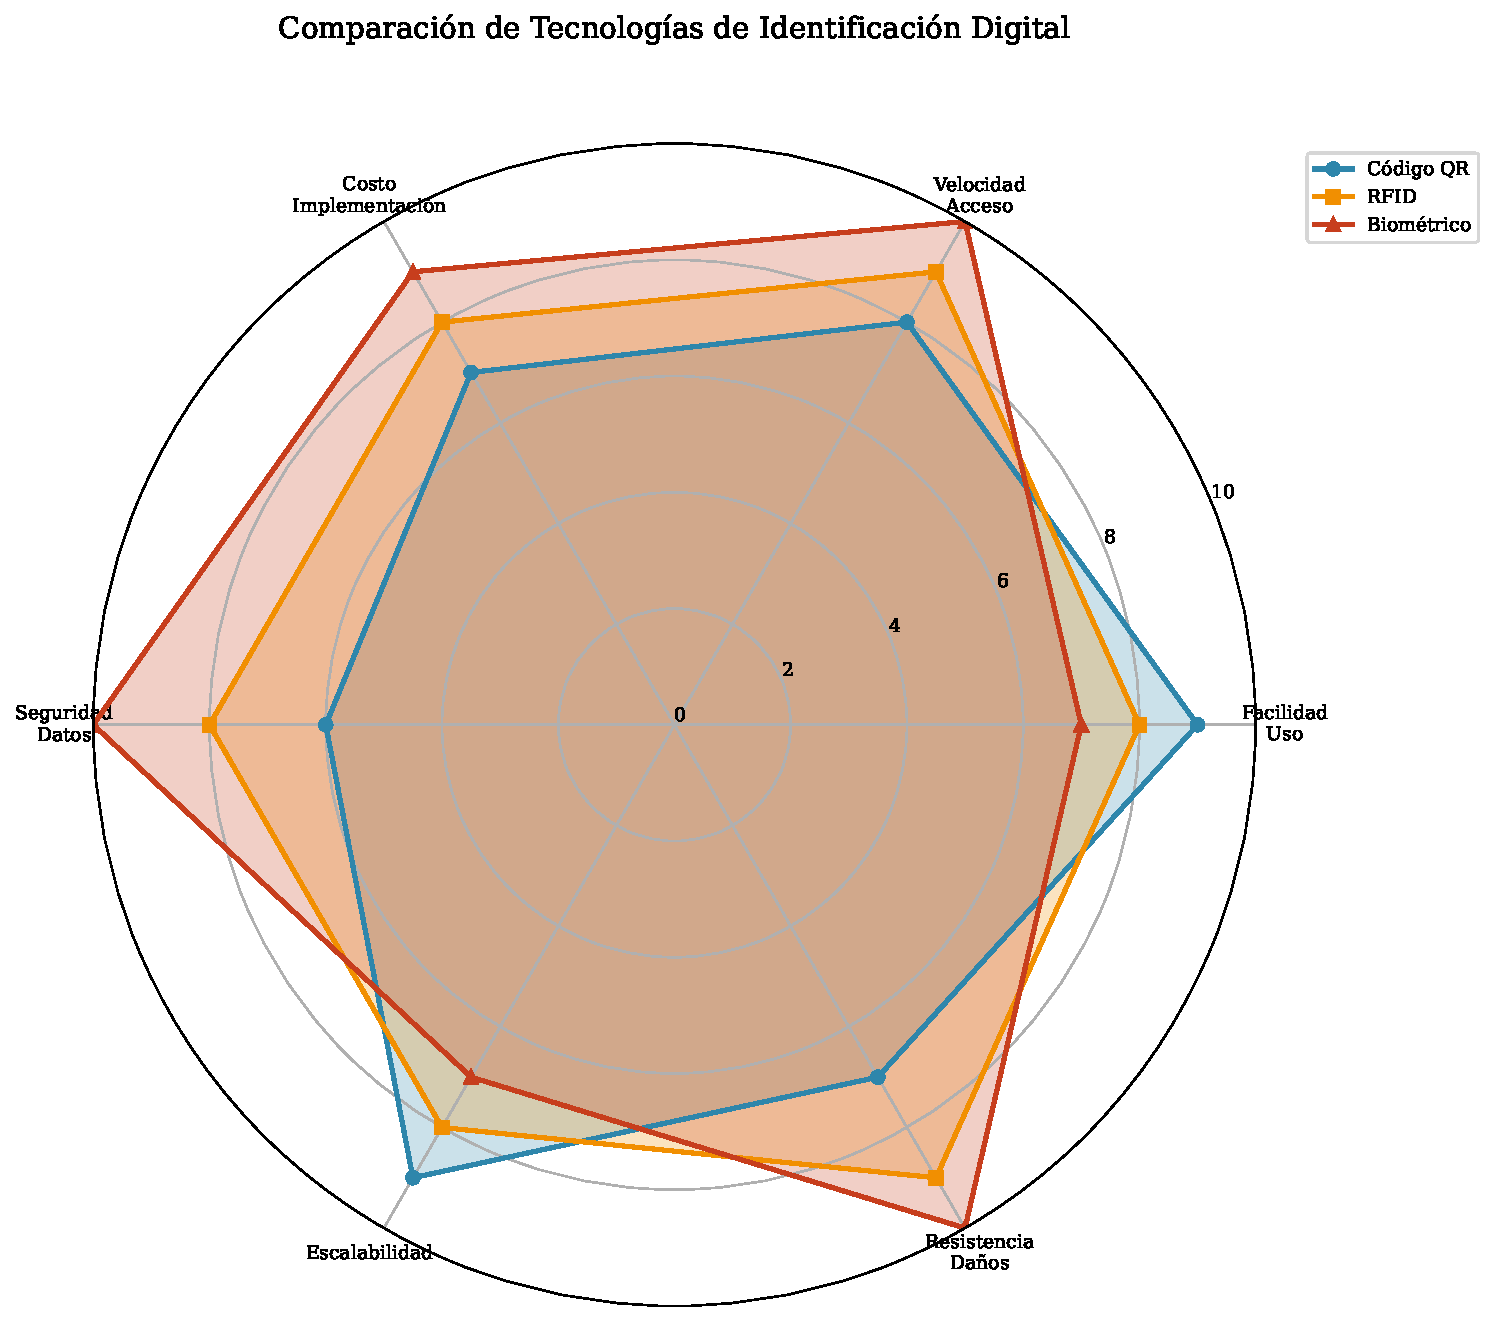
\includegraphics[width=0.45\textwidth]{graphics/comparacion_tecnologias.pdf}
\caption{Comparación multi-criterio de tecnologías de identificación digital: QR, RFID y Biométrico}
\label{fig:comparacion_tecnologias}
\end{figure}

\section{5. Resultados observados en distintas experiencias}

\subsection{5.1. A nivel operativo}

Varios estudios y experiencias registradas coinciden en que:

El ingreso se acelera notablemente.

Se reducen filas y demoras.

Los registros dejan de depender de la memoria o buena voluntad de alguien.

La información es más precisa y fácil de auditar.

Los informes se generan solos y con datos completos.

Esto facilita procesos administrativos que antes tomaban horas o requerían revisar cientos de registros manuales.

\subsection{5.2. Impacto en estudiantes y usuarios}

En contextos educativos, los QR integrados en guías, documentos o cursos también mejoran el aprendizaje. Los estudiantes acceden a videos, materiales o ejercicios con solo escanear. En general, los usuarios reportan que el proceso es más cómodo, práctico y menos tedioso.

\begin{figure}[H]
\centering
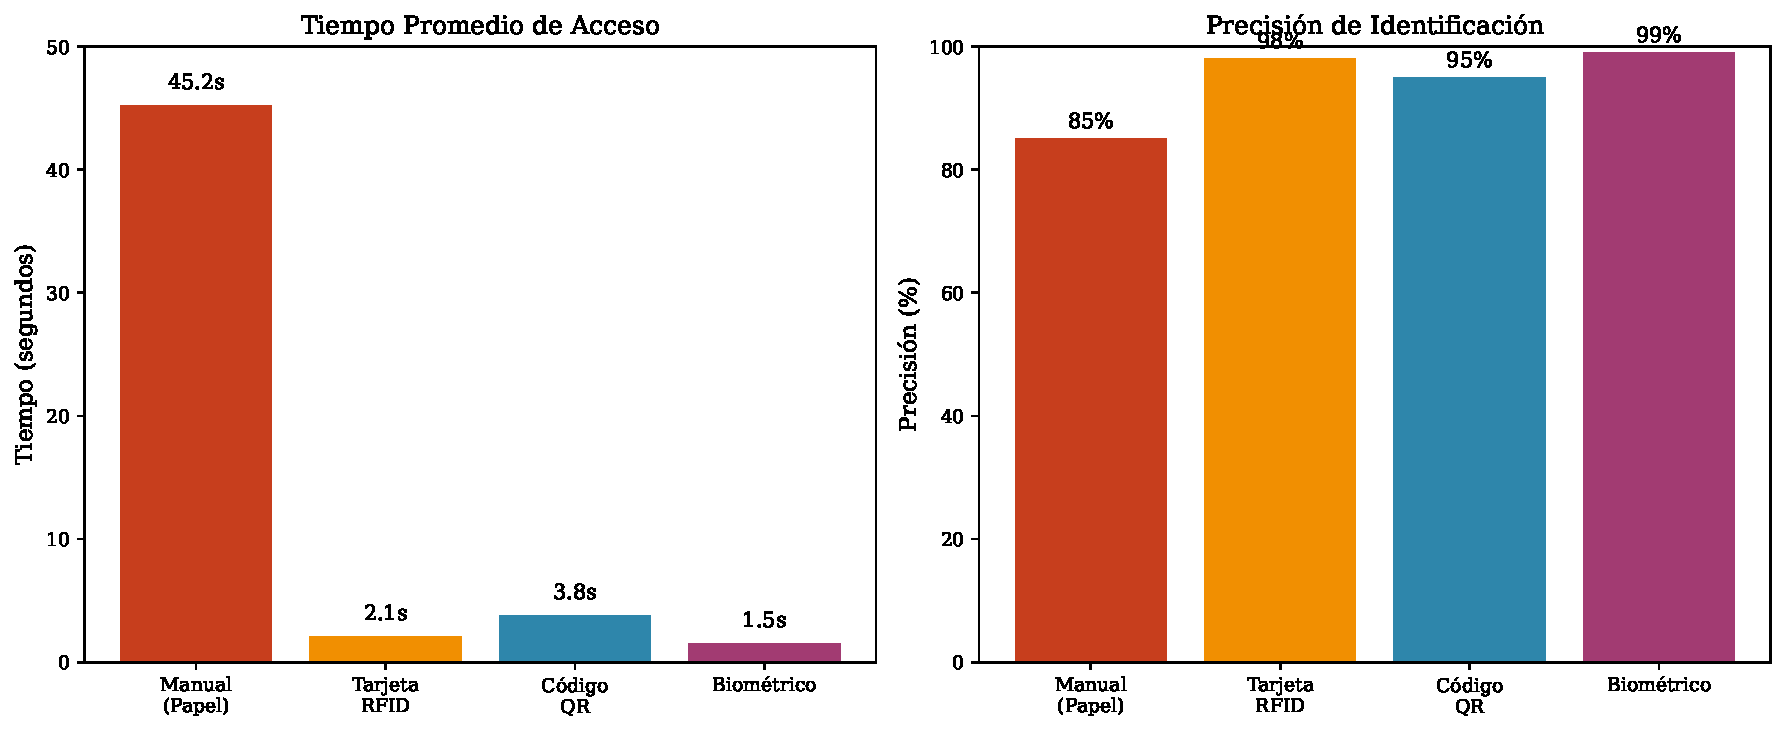
\includegraphics[width=0.48\textwidth]{graphics/eficiencia_acceso.pdf}
\caption{Tiempo promedio de acceso y precisión de identificación por método}
\label{fig:eficiencia_acceso}
\end{figure}

\begin{figure}[H]
\centering
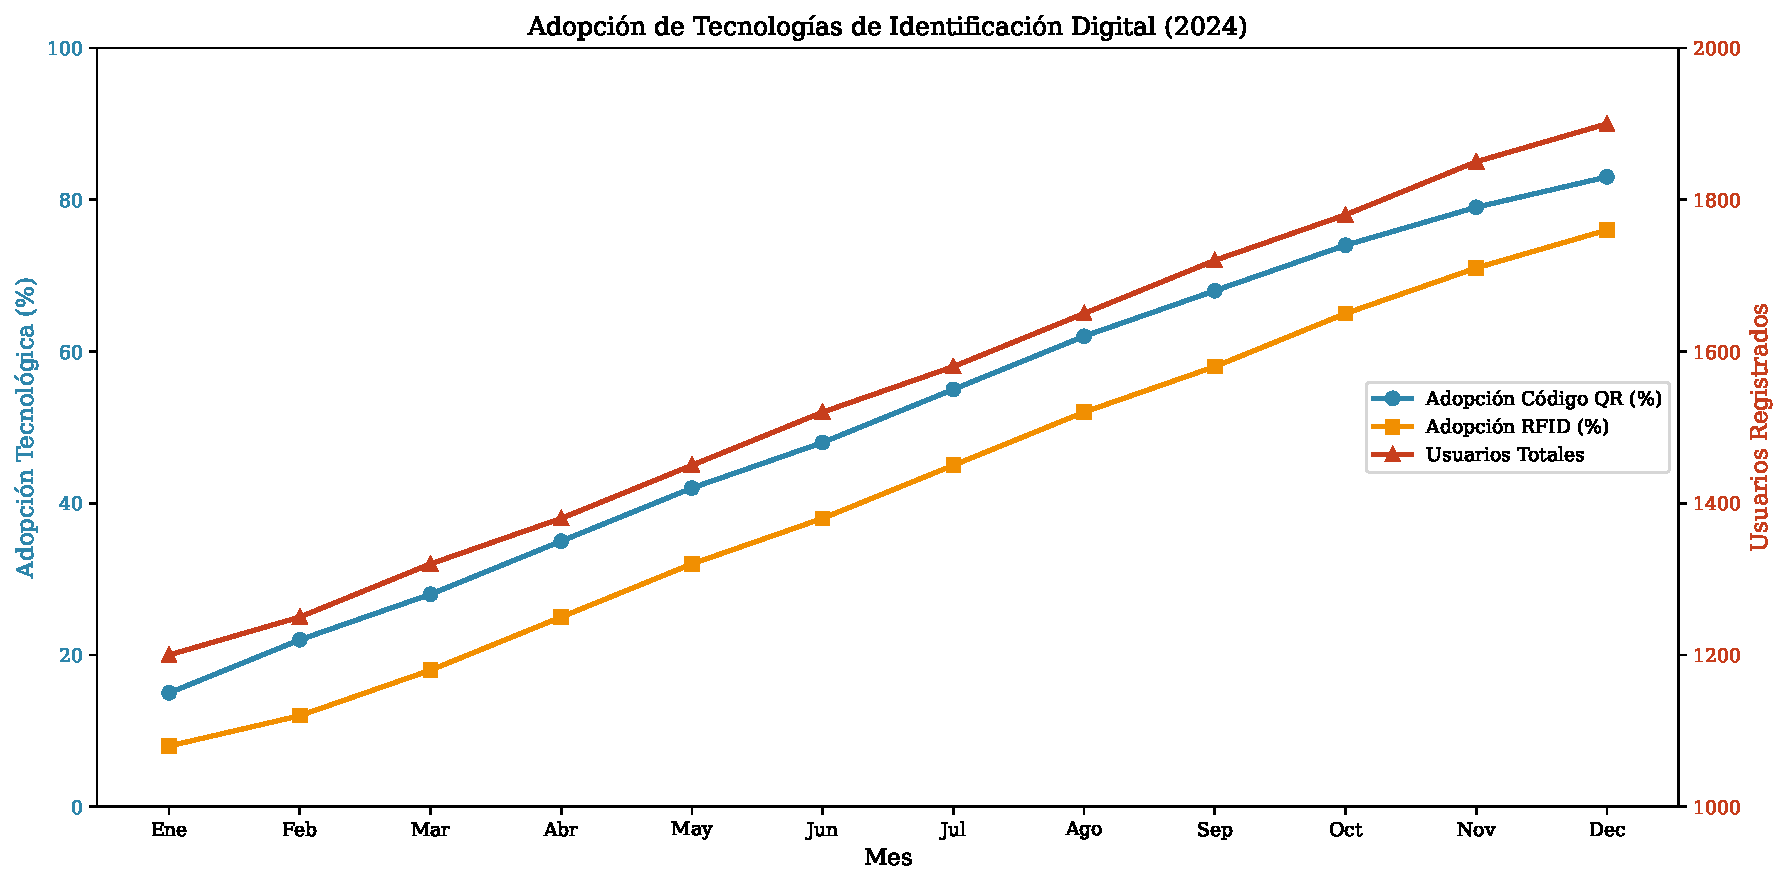
\includegraphics[width=0.48\textwidth]{graphics/adopcion_tecnologias.pdf}
\caption{Evolución de la adopción de tecnologías QR y RFID (2024)}
\label{fig:adopcion_tecnologias}
\end{figure}

\section{6. Problemas que aparecen (y que muchas veces no se mencionan)}

\subsection{6.1. Escalabilidad}

Uno de los mayores desafíos es que el sistema debe responder igual de bien cuando entran 10 personas que cuando entran 2.000 al mismo tiempo. Si la infraestructura no soporta la carga, se generan filas, caídas en la red e incluso registros incompletos.

Esto obliga a pensar seriamente en:

Capacidad de servidores.

Velocidad del procesamiento.

Red interna.

Sincronización entre dispositivos.

Un sistema que funciona bien en días tranquilos puede colapsar en hora pico.

\subsection{6.2. Privacidad y manejo ético}

La información que se maneja es muy sensible. Saber cuándo entra y sale una persona puede revelar patrones de comportamiento. Por eso, la seguridad no se puede reducir a un simple cifrado; se requieren políticas claras de almacenamiento, acceso, eliminación y auditoría.

\subsection{6.3. Integración con otros sistemas}

El control de acceso por sí solo no basta. Muchas instituciones necesitan cruzar esos datos con horarios de clase, registros de empleados, áreas restringidas, sistemas de emergencia y bases de datos académicas.

Cuando las integraciones no están bien diseñadas, los datos se pierden, se duplican o se vuelven contradictorios.

\begin{figure}[H]
\centering
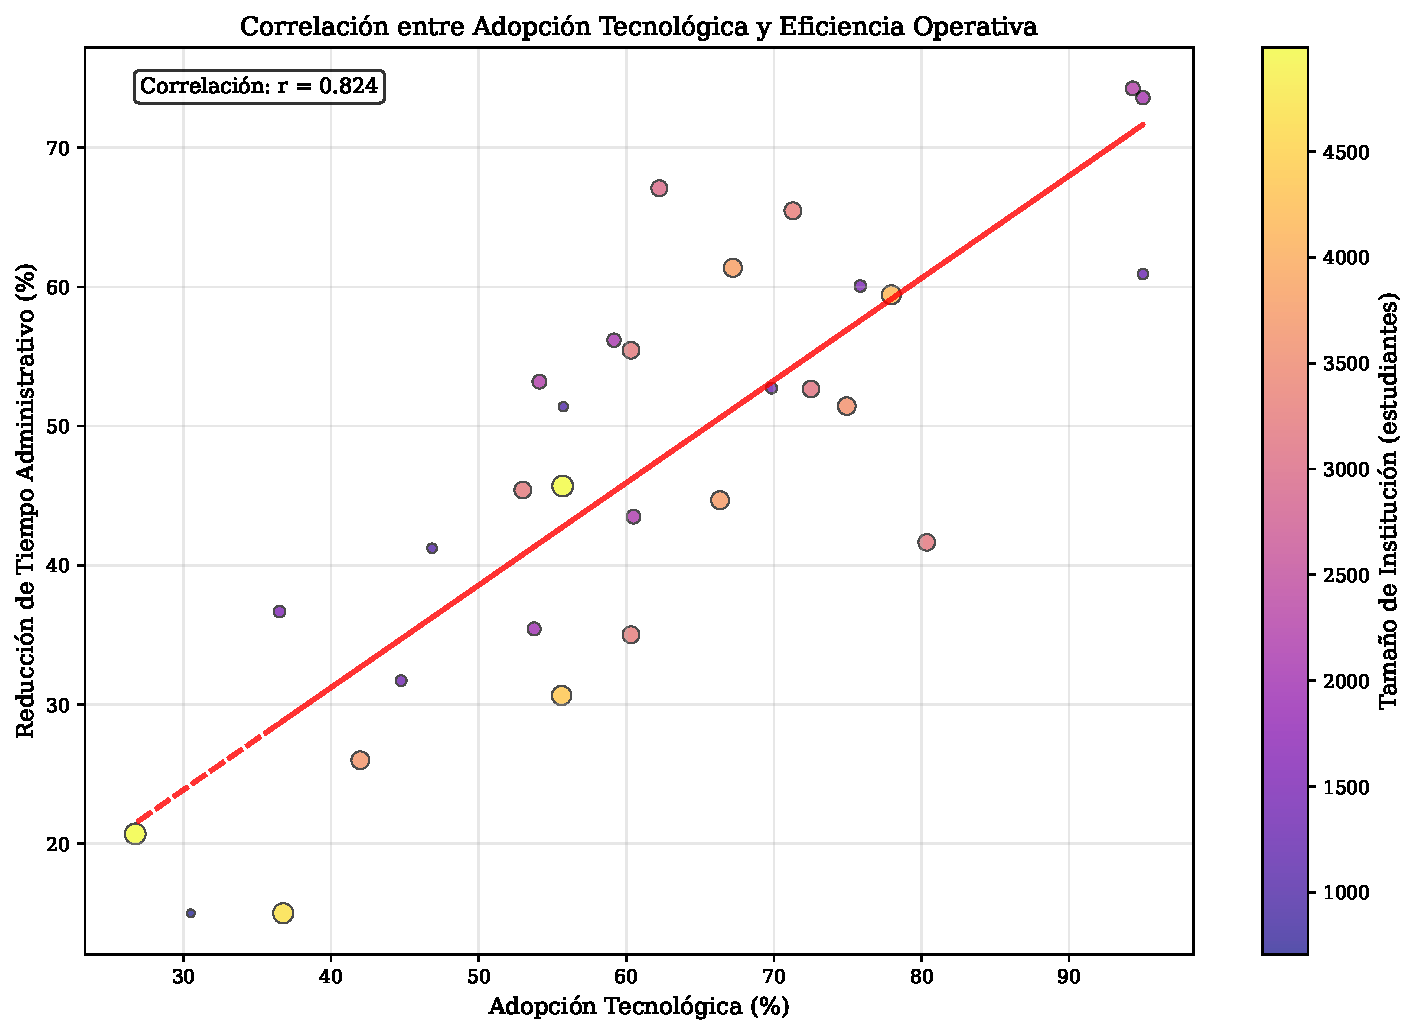
\includegraphics[width=0.46\textwidth]{graphics/correlacion_tecnologias.pdf}
\caption{Correlación entre adopción tecnológica y reducción de tiempo administrativo}
\label{fig:correlacion_tecnologias}
\end{figure}

\section{7. Conclusiones finales (tono reflexivo y humano)}

Los códigos QR y los sistemas RFID han demostrado ser herramientas valiosas para modernizar procesos que durante años se hicieron manualmente. No son soluciones mágicas, pero sí representan un paso importante hacia instituciones más organizadas, eficientes y capaces de tomar decisiones basadas en datos reales.

Al implementar estas tecnologías, las instituciones no solo ganan rapidez; también construyen un sistema más transparente, más seguro y más útil para estudiantes, empleados y administradores.

Aun así, el reto está en implementarlas bien: proteger la privacidad, asegurar que el sistema no colapse en horas críticas y garantizar que todos los módulos se comuniquen correctamente.

\end{document}